%----------------------------------------------------------------------------------------
%	Introduction PAGE
%----------------------------------------------------------------------------------------

%\addchaptertocentry{Introduction}

%\newpage

%{\huge\textbf{Introduction}\par}
%\HRule \\[0.4cm] % Horizontal line

\chapter{Introduction}
\label{chapter:intro}
\noindent\makebox[\linewidth]{\rule{0.75\paperwidth}{0.4pt}}
\noindent\makebox[\linewidth]{\rule{0.75\paperwidth}{0.4pt}}

\localtableofcontents % local toc

\noindent\makebox[\linewidth]{\rule{0.75\paperwidth}{0.4pt}}
\noindent\makebox[\linewidth]{\rule{0.75\paperwidth}{0.4pt}}

\newpage
%----------------------------------------------------------------------------------------

\section{Context of the thesis}
%\textbf{Keywords:} Brain Imaging, Neuroscience Neurons, cells, Clinical work, cognitive science\\
%=> Non-invasive techniques/scanning - fMRI, M/\ac{eeg} (functional)\\
%=> Why it is important to get back (inverse problem) to the brain? Ex: Epilepsy for clinical case or more how the brain works for a cognitive task.

Understanding the full complexity of the brain has been a challenging research project for decades, yet there are many mysteries that remain unsolved.
Being able to model how the brain represents, analyzes, processes, and transforms information of millions of different tasks in a record time is primordial for both cognitive and clinical studies. These tasks can go from language, perception, memory, attention, emotion, to reasoning and creativity. Studying the behavior of the brain at each task and extracting information to define its involved network will result in a better understanding of its functions. This has been widely used in other fields such as Artificial Intelligence where scientists and engineers try to implement aspects they learned from the human brain in computers. Unlike the cognitive science questions, in the clinical diagnostic, understanding how a pathology is affecting the brain helps to find a cure or a way to improve patients' life. For example, being able to detect autism in early age of childhood helps the parents to provide a specific education and a better future.\\

To make this brain scanning possible, several cutting-edge technologies are used  depending on the question one is asking. These techniques differ from their degree of invasiveness, and their spatial and temporal resolutions as it can be seen in Figure~\ref{fig:brain_imaging_techniques}.
For the different tasks I mentioned above, one very important aspect is time. The brain is able to process most of the tasks in a fraction of a second, for example to recognize an emotion, to perceive a familiar face, etc. In this thesis, to study this high temporal resolution of the brain, I was interested in two direct brain imaging techniques.

\begin{figure}
	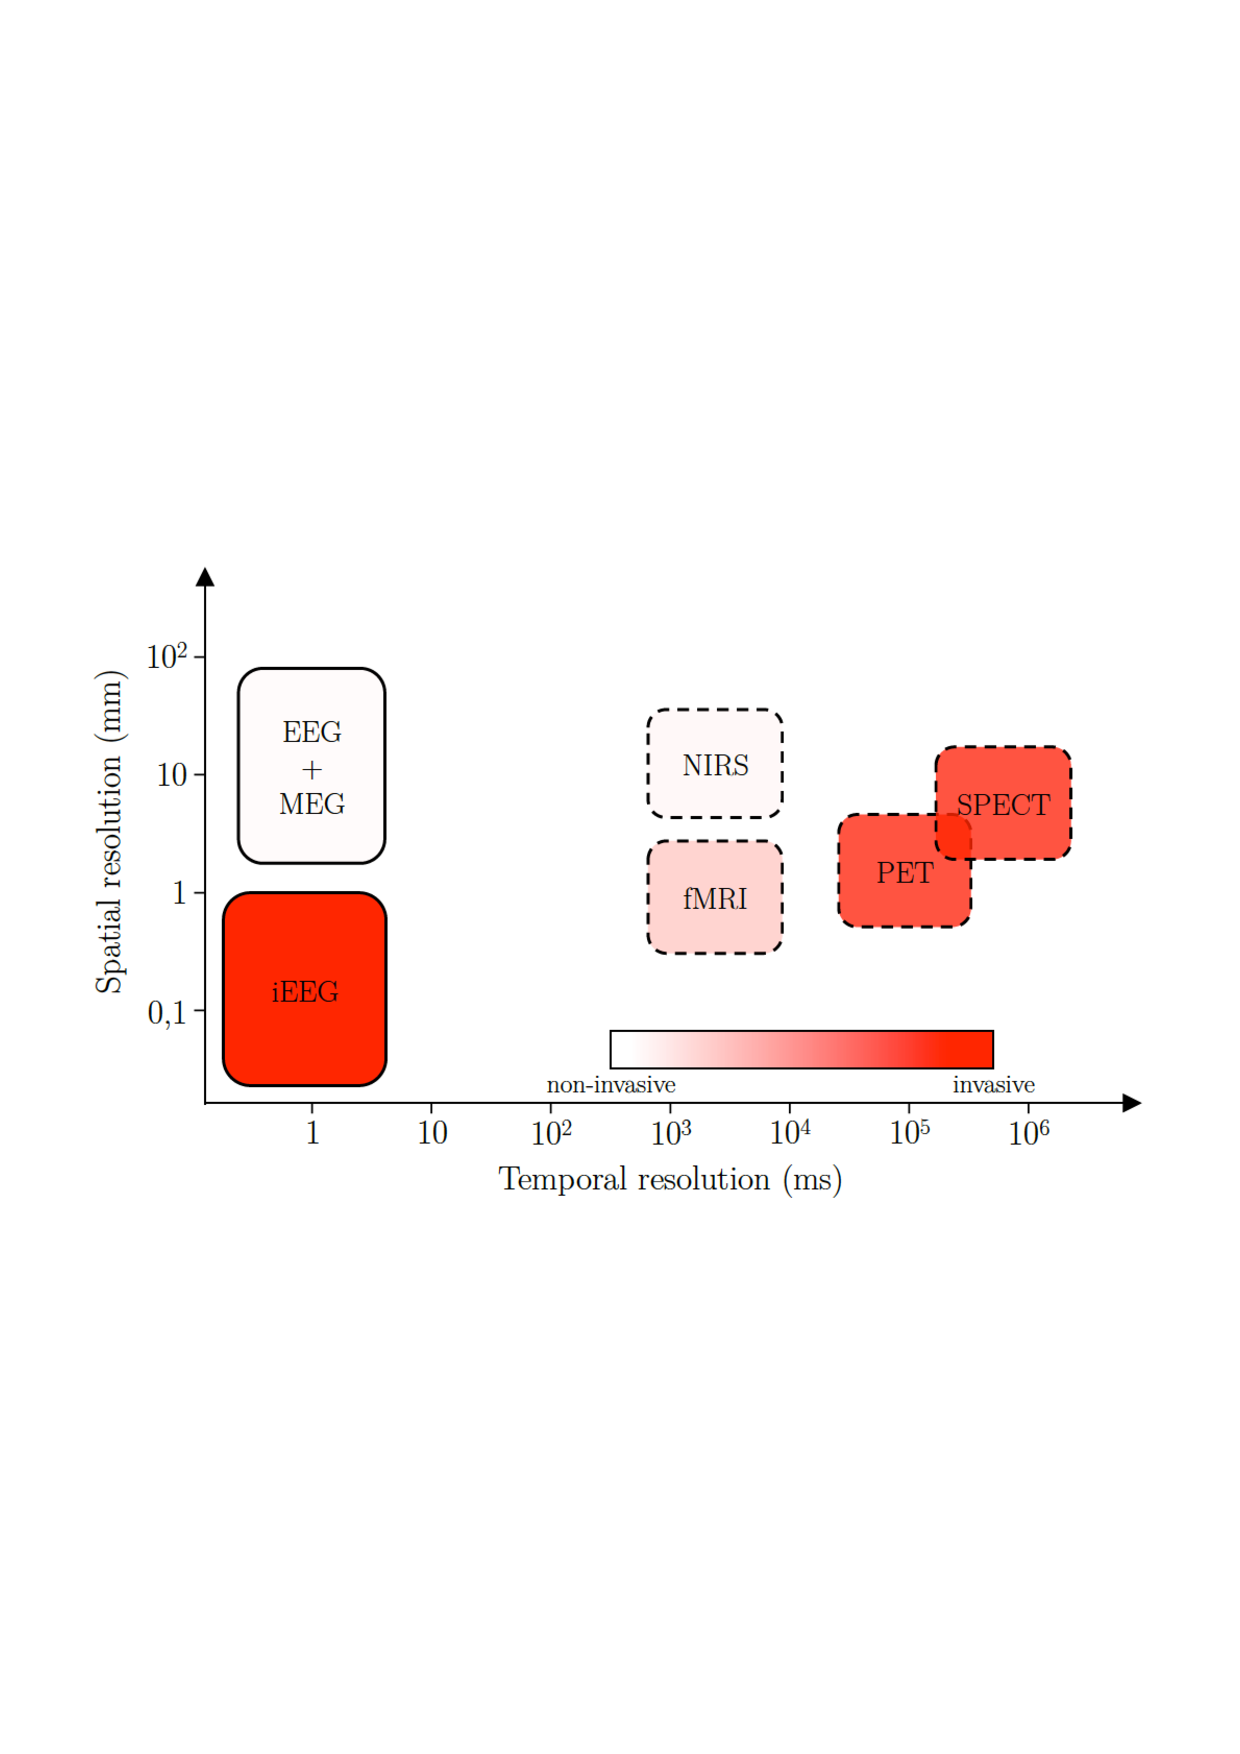
\includegraphics[trim={1cm 8cm 2cm 10cm},width=0.95\textwidth]{introduction/brain_imaging_techniques}
    \caption{Overview of spatial and temporal resolutions of different functional neuroimaging methods. Direct approaches (\ac{eeg}, i\ac{eeg}, \ac{meg}) are indicated by solid boxes and indirect approaches (\ac{fMRI}, \ac{NIRS}, \ac{PET}, and \ac{SPECT}) by dashed boxes. The colors of the boxes indicate the degree of invasiveness.
    }
    \label{fig:brain_imaging_techniques}
\end{figure}
 
\Ac{meg} and \ac{eeg} are functional neuro-imaging techniques for mapping the brain activity. They respectively record the magnetic and electric fields produced by electrical currents naturally occurring in the brain within the neurons. They use an array of sensors positioned over the scalp that are extremely sensitive to minuscule changes in the magnetic field (measured by \ac{meg}) produced by small changes in the electrical activity (measured by \ac{eeg}) within the brain. It is, therefore, a direct measurement of neural activity. \ac{meg}/\ac{eeg} as a technique for investigating the neural function in the brain is not new but was originally pioneered in the late 1960s. However, it is only since the early 1990s, with the introduction of high density detector grids covering the whole head, that the full potential of \ac{meg} has begun to be realized. The biggest advantage of \ac{meg} and \ac{eeg}, compared to \ac{fMRI} which is much more established in the neuroscience research, is the time resolution. In fMRI, the neuronal activation is indirectly measured via local changes in the level of blood oxygenation, and a long time window is typically compressed in one measured brain volume. The other techniques mentioned in Figure~\ref{fig:brain_imaging_techniques} are also indirect functional brain imaging techniques.\\

Using very sensitive magnetometers/electrodes (sensors), \ac{meg} and \ac{eeg} deliver insight into the brain activity with high temporal and good spatial resolution. They allow the measurements of the ongoing activity which describe the active brain sources' state at each millisecond. This problem of estimating the result of the measurements is called \textit{forward problem}. The bioelectromagnetic forward problem describes the relationship between a given neural activity in the brain and the observable \ac{meg} and \ac{eeg} signals. Its solution models mathematically the neural activity, the volume conductor, and the measurement setup. It allows us to link the scalp potentials and external fields given an internal current distribution by a stable and unique solution, which is thus a well-posed problem. \\

Its counterpart, the bioelectromagnetic \textit{inverse problem}, consists in using the actual measurements to infer the parameters (locations, amplitude, orientations) giving the distribution of the neural generators. It is an ill-posed problem in the sense of Hadamard due to its non-uniqueness and high sensitivity to noise, which makes its solution unstable. The inverse problem is the so called $n \ll p$ problem in machine learning, where you have much more unknowns $p$ to be estimated than the number of observations or variables $n$. This problem has infinite solution, mainly due to the small number of sensors (obervations $n$) present in the \ac{meg} and \ac{eeg}. Actually, even if the \ac{meg} and \ac{eeg} were measured simultaneously at infinitely many points over the head, the information would still be insufficient to uniquely compute the brain source distribution that generated the measured brain signals. This is due to the fact that there are different combinations of sources able to cause \textit{exactly} the same potential fields on the head. Thus, to infer the neural activity generating the data at the sensor level, different source reconstruction techniques can be applied, which typically employ a priori knowledge on the state of the brain activity in order to reduce the set of solutions to a unique one.\\

In the past twenty years, several lines of research have emerged to tackle the problem. The most common approach widely used in clinical application is the \ac{ECD}, which assumes the underlying neural sources to be focal, as for epileptic study. The limitation of the dipole fitting technique is its non-linearity, which makes the reconstruction challenging. Also, there are difficulties to accurately estimate the correct number of dipoles in advance. \\

Unlike the dipole fitting method, distributed source models divide the source space into a grid containing a large number of possible dipoles (ECDs). The reconstruction of the source space is done simultaneously over all ECDs, which is less challenging when having correlated sources. However due to the large number of dipoles, the corresponding regression problem is undertermined, and then requires regularization. The regularization will define the type of a priori one needs to put on the solution, such as structural information, spatio-temporal characteristics of the source estimate. The disadvantage of these models compared to dipole fitting is that the solution is smeared, meaning it is not focal, so harder to interpret.\\

Nevertheless, the sparsity in the solution can be promoted with a specific type of regularization in the regression model. Sparse models are actually the main interest of this thesis. They have been proposed in other fields of research and are widely used. In the signal processing literature, various signals can be defined as the linear combination of basis vectors, called \textit{atoms}. This technique is also known as compressed sensing. These atoms are defined in a fix overcomplete dictionary; the underlying motivation is that even though the observed signal lies in a high-dimensional space, the actual signal is organized in a lower-dimensional space. This property has been used in the audio domain, specifically in the analysis of speech, sounds, and music, \textit{e.g.} in order to classify a sound sample. The idea of sparse decomposition is also behind the JPEG2000 compression, which aims to keep only a few atoms best approximating the image. More in the image processing literature, the sparse models were used for denoising and image reconstruction (\ac{MRI},...). They are also linked to the dictionary learning literature, where one tries to learn a redundant and overcomplete dictionary, which makes it possible to reconstruct a signal/image using a sparse setting.\\

\section{Objective and scope}
%\textbf{Keywords:} Not only solve the IP but improve methods from the start to the end of the problem of source localization\\
%=> Sparse solutions (references), what people have been doing and how do we choosed to handle the problem\\
%=> Hyperparameter estimatio, to improve the tuning of the parameters which is important for solving the problem accurately.

In this thesis, I have been interested in sparse models to reconstruct the source estimate for \ac{meg} and \ac{eeg} applications. Obtaining acceptable solutions, easy to interpret, does not depend only on the a priori knownledge we impose, but several questions might be asked:
\begin{itemize}
\item How do we best fix the regularization to promote sparsity, in such a way to obtain interpretable source estimates?
\item How do we set the hyperparameters of the regression problem?
\item How do we quantify the uncertainty of these models?
\item How do we objectively compare the different state of the art solvers?
\end{itemize}
These points define the scope of this thesis. It tries to firstly tackle the problem of non-stationary sources, \textit{i.e.}, how to estimate a source that has a neuroscientific explanation as being active during a short time window only, when studying a longer window. This involves the formulation of the problem in the time-frequency domain, which needs to explicit the dictionary of the decomposition. Secondly, this thesis tries to find a way to automatically estimate the hyperparameter of the regression model to make comparison between solvers easier. The next step was to rewrite the problem as done by other communities in a Bayesian formulation. This gave a way to bridge the gap between the variational and the Bayesian worlds by writing down their equivalence under a specific parametrization of the same problem. The advantage of the Bayesian formulation is the ability to investigate the posterior distribution, making a study of the solution's uncertainty possible. This involves the presentation of \ac{MCMC} algorithms to sample from the posterior distribution. A third and last project of this thesis was to put together all the actual knowledge on source localization in \ac{meg}/\ac{eeg} and have a complete study of their reconstruction on a phantom dataset.

\section{Contributions of the author}
This thesis presents novel approaches for source reconstruction in \ac{meg}/\ac{eeg}. It can be divided into four main projects:
\begin{itemize}
\item The implementation of a widely known algorithm for the \ac{meg}/\ac{eeg} inverse problem, called Recursively Applied and Projected (RAP) MUSIC~\cite{mosher-leahy:1999}. The aim was to have a comparison with a state of the art sparse solver based on a non-convex regularization which promotes more sparsity by getting rid of all spurious sources. This work has been published in the \textbf{IEEE Transactions on Medical Imaging (TMI)}~\cite{strohmeier-etal:16}.

\item The improvement of a previous work by Daniel Strohmeier on source reconstruction in the time frequency domain, which resulted in the introduction of the TF-MxNE  (Time-Frequency mixed-norm) algorithm. The contribution tackles the problem of choosing the dictionary where to decompose the data when working in the time-frequency domain. This consists on enabling the possibility to use combined dictionaries to make the algorithm able to find both transient and longer waveforms present in the brain signal. This work has been published in the IEEE workshop on \textbf{Pattern Recognition in NeuroImaging (PRNI)}~\cite{bekhti2016m}.

\item Different lines of research to solve the \ac{meg}/\ac{eeg} inverse problem gave different formulations. The mostly used formulation in this thesis is a regularized regression model as done in most machine learning problems. With this type of models, one needs to find a good compromise between the term that tries to fit the data called the data fit, and the term regularizing the problem which takes into account any assumption one has onto the problem. This compromise is controlled by an external parameter usually called hyperparameter. For a practical example, when using sparse regularization, if this hyperparameter is fixed to a small value, \textit{i.e.} the regularization term is not as important as the data fit, then the resulting solution will not be sparse enough and vice versa. Thus, the second contribution of this thesis was then to find an automated way to estimate this hypermarameter under some conditions of the model. This work has been published in the \textbf{European Signal Processing Conference (EUSIPCO)}~\cite{bekhti_eusipco}.

\item The biggest drawback of the sparse solvers is the fact that they give one solution without any estimation of variance or any kind of confidence interval. Some other application areas make use of Bayesian inference, mainly because it allows the estimation of uncertainty and its quantification is paramount. Therefore, the third contribution of this thesis is to rewrite to problem as done in a Bayesian world, and tries to bridge this formulation with what has been presented so far. This project shows that under some conditions, the Bayesian formulation and the variational one are equivalent. Then, it shows how we can take advantage of the posterior distribution to extract uncertainty maps. This work has been submitted and is under review in the \textbf{journal Physics in Medicine \& Biology (PMB)}~\cite{bekhti_arxiv_pmb}.

\item The final project of this thesis is to test and validate our solvers and several other ones that are the mostly used at this day for neuroscience applications. This is done on a phantom dataset which is a simulated dataset with a realistic environment similar to a real humain brain. This work should be submitted soon to a journal paper.

\item An extra project on brain decoding is presented at the end of this thesis. This work presents a novel approach based on a ridge regression with a specific metric that takes ordered target into account. The approach is novel in terms of application to \ac{meg} data. This work has been submitted and is under review in the journal \textbf{Plos One}~\cite{Bekhti_bioarxiv}.

\item The implementation of some of the contributions is already on the MNE-Python package~\cite{mne,mne-python}, the others should also be integrated soon. Another contribution with a coworker's project is published in both \textbf{Pattern Recognition in NeuroImaging}~\cite{jas_autoreject_prni} and \textbf{Neuroimage}~\cite{jas_neuroimage}.
\end{itemize}

\section{Structure of the thesis}
\begin{itemize}
\item \textbf{Chapter 2: Background and work related to the
MEG/\ac{eeg} inverse problem}\\
This chapter defines the basics and the background needed for what will be presented in the rest of this thesis. It starts by giving the origin of the \ac{meg} and \ac{eeg} recordings, \textit{i.e.}, what do the techniques really measure? It gives then more insight on the forward operator and how it is computed efficiently. At this stage, I present a full state of the art of inverse problems defining the three main approaches: beamforming or scanning techniques, image-based methods with distributed models, and sparse source models. Afterwards, I present some basics of time-frequency decomposition, and compare several dictionaries by giving their advantages. I finish this chapter by an optimization section, defining different ways to regularize the ill-posed problem and then how do we solve them. It also gives a comparison between several solvers.\\

\item \textbf{Chapter 3: Source localization with multi-scale dictionaries}\\
This chapter is dedicated to our first contribution, \textit{i.e.} solving the inverse problem in the time-frequency domain using a multi-scale dictionary. 
Source localization in the time-frequency domain has already been investigated using a Gabor dictionary in a convex~\cite{Gramfort_Strohmeier_Haueisen_Hamalainen_Kowalski13} and a non-convex way~\cite{Strohmeier-etal:2015}. However, the choice of an optimal dictionary remains unsolved. Due to a mixture of signals, i.e. short transient signals (right after the stimulus onset) and slower brain waves, the choice of a single dictionary simultaneously explaining both signals types in a sparse way is difficult. This chapter introduces a method to improve the source estimation relying on a multi-scale dictionary, i.e. multiple dictionaries with different scales concatenated to fit short transients and slow waves at the same time. The benefits of this approach are shown in terms of reduced leakage (time courses mixture), temporal smoothness and detection of both signals types.

%Finally, the last chapter shows the experimental results obtained on simulated and on real \ac{meg} data. Then we discuss the achievements of this thesis and future work. 
%http://imaging.mrc-cbu.cam.ac.uk/\ac{meg}/Intro\ac{eeg}\ac{meg}

\item \textbf{Chapter 4: The Bayesian approach: Hierarchical Bayesian modeling}\\
This chapter gives the basic concepts of the Bayesian formulation of the \ac{meg}/\ac{eeg} inverse problem. It also aims to explain the different jargon to link the variational and the Bayesian definitions. This ends up in defining an equivalence between the two communities under some conditions, while taking advantage of the Bayesian formulation which enables us to study the multiple modes of the posterior distribution. The modes of the posterior will define several possible solutions to the inverse problem, allowing then the obtention of uncertainty maps of the source estimates. 

\item \textbf{Chapter 5: Benchmarking on phantom datasets}\\
This chapter is a validation chapter on a phantom dataset. Phantom data is a dataset obtained by measuring the \ac{meg}/\ac{eeg} activity with a humain skull phantom head. All real aspects of a head are simulated to generate the same conductivity which is expected with a real skull. The dataset shown in this chapter has four simulated dipoles at different depth. With the knowledge of the groundtruth, this chapter investigates the efficiency of each solver in terms of source localization, orientation and amplitude.

\item \textbf{Chapter 6: Decoding visual motion from \ac{meg}}\\
This chapter illustrates an extra project outside of the inverse problem topic. It is based on an application of machine learning to neuroscience. The aim was to develop an efficient approach to decode brain activity recorded with \ac{meg} while participants discriminated the coherence of two intermingled clouds of dots.
\end{itemize}

\newpage
\section{Publications of the author}
\subsection*{Peer-reviewed journal papers:}

\begin{itemize}
\item \textbf{Y. bekhti}, and A. Gramfort, "Validation of dipole localization using phantom data in \ac{meg} source imaging," in preparation.
\item \textbf{Y. Bekhti}, F. Lucka, J. Salmon, and A. Gramfort, "A hierarchical Bayesian perspective on majorization-minimization for non-convex sparse regression: application to M/\ac{eeg} source imaging," IEEE Physics in Medicine \& Biology, (submitted).
\item \textbf{Y. Bekhti}, A. Gramfort, N. Zilber, and V. van Wassenhove, "Decoding the categorization of visual motion with magnetoencephalography," Plos One, (submitted).
\item D. Strohmeier, \textbf{Y. Bekhti}, J. Haueisen, and A. Gramfort, "The iterative reweighted Mixed-Norm Estimate for spatio-temporal \ac{meg}/\ac{eeg} source reconstruction," IEEE Transactions on Medical Imaging, vol. 35, no. 10, pp. 2218-2228, 2016.
\item M. Jas, D.A. Engemann, \textbf{Y. Bekhti}, F. Raimondo, and A. Gramfort, "Autoreject: Automated artifact rejection for \ac{meg} and \ac{eeg} data," NeuroImage, vol. 159, pp. 417-429, 2016.
\end{itemize}

\subsection*{Peer-reviewed conference papers:}
\begin{itemize}
\item \textbf{Y. Bekhti}, R. Badeau, and A. Gramfort, "Hyperparameter estimation in maximum a posteriori regression using group sparsity with an application to brain imaging," Signal Processing Conference (EUSIPCO), pp. 246-250, 2017.
\item \textbf{Y. Bekhti}, D. Strohmeier, M. Jas, R. Badeau, and A. Gramfort, "M/\ac{eeg} source localization with multi-scale time-frequency dictionaries," International workshop on Pattern Recognition in NeuroImaging (PRNI), pp. 1-4, 2016.
\item M. Jas, D.A. Engemann, F. Raimondo, \textbf{Y. Bekhti}, and A Gramfort, "Automated rejection and repair of bad trials in \ac{meg}/\ac{eeg}", International workshop on Pattern Recognition in NeuroImaging (PRNI), pp. 1-4, 2016.
\end{itemize}
